%!TEX root = ../main.tex
\section{Rested rotting bandit: model and preliminaries}
\label{sec:rested-model}

\subsubsection*{Feedback loop}
At each round $t$, an agent chooses an arm $i_t \in \possibleArms \triangleq \left\{ 1, ... , K\right\} $ and receives a noisy reward $o_t$. The reward associated to each arm $i$ is a $\subgaussian^2$-sub-gaussian random variable with expected value of $\mu_i(n)$, which depends on the number of times $n$ it was pulled before; $\mu_i(0)$ is the initial expected value.
We use $\mu_i(n)$ for the expected value of arm~$i$ \textit{after $n$ pulls} instead of when it is pulled \textit{for the $n$-th time}. 
Let $\historyt \triangleq \left\{ \left\{ i_s, o_s \right\}, \forall s < t \right\}$ be the sequence of arms pulled and rewards observed until round $t$, then 
%
\begin{equation}
\label{eq:rested-feedback}
o_{t} \triangleq \mu_{i_t}(N_{i_t,t-1}) + \noise_t
 \;\; \text{with}\; \EE{ \noise_t | \historyt }= 0 \;\; \text{and} \; \forall \lambda \in \R, \; \EE{ e^{\lambda\noise_t}} \leq e^{\frac{\subgaussian\lambda^2}{2}},
\end{equation}
%
where $N_{i,t}\triangleq \sum_{s\!=\!1}^{t} \mathbb{I}\{i_s \!=\! i\}$ is the number of times arm $i$ is pulled after round $t$.
\begin{definition}\label{def:rew-bounded-decay} 
We introduce $\rewardSet$, the set of non-increasing reward functions with bounded decay $L$,
\[ 
\rewardSet \triangleq \left\{ \mu : \NN \rightarrow \left[- \infty,  L\right] \;\big{|}\; 0 \leq \mu(n) - \mu(n+1)  \leq L \text{ and } \mu(0) \in \left[0,  L\right] \right\}.
\]
\end{definition}
%
\begin{remark}
We define the set of constant reward functions in $\left[0, L\right]$: 
\[ 
\stationarySet \triangleq \left\{ \mu : \NN \rightarrow \left[0,  L\right] \;\big{|}\;  \mu(n) = \mu_i  \right\}.
\]
We have that $\stationarySet \subset \rewardSet$. Hence, we can conclude that the rotting bandits model includes all the stationary bandits problems.
\end{remark}
%
\subsubsection*{Online and offline objectives}
In this chapter, we will only consider deterministic agents which output an arm $i$ at each round $t$. They are degenerate cases of probabilistic agents, which outputs a probability distribution over arms at each round. For the sake of simplicity, we present only the deterministic formalism.   

We will distinguish two types of policies. On the one hand, an offline (or oracle) policy~$\pi \in \PiO$ is a function which maps the round $t$ and the set of reward functions $\mu \triangleq \left\{ \mu_i \right\}_{i \in \possibleArms}$ to arms, i.e. $\pi(t, \mu) \in \possibleArms$.  On the other hand, an online (or learning) policy~$\pi \in \PiL$ is a function from the history of observations at time $t$ (which includes the knowledge of the round $t$) to arms, i.e., $\pi(\mathcal{H}_t) \in \mathcal{K}$. For both types of policies, we often use the shorter notation $\pi(t)$, where the dependencies on $\mu$ or $\mathcal{H}_t$ is implicit. 

For a policy $\pi$, let $N_{i,t}^\pi \triangleq \sum_{s=1}^{t} \mathbb{I}\{\pi(s) = i\}$ be the number of pulls of arm $i$ at the end of round $t$. The performance of a policy $\pi$ is measured by the (conditionally expected) rewards accumulated over time, 
%
\begin{equation}
\label{eq:cumul-reward-rested}
J_T(\pi) \triangleq \sum_{t=1}^T \mu_{\pi(t)}\pa{N_{\pi(t),t-1}} = \sum_{i \in \possibleArms} \sum_{n=0}^{N_{i,T}^\pi-1} \mu_i(n).
\end{equation}
%
\begin{remark}
The cumulative reward depends only on the number of pulls of each arm at the horizon $T$: it does not depend on the specific pulling order of the arms. Hence, two distinct policies with the same pulling allocation at the horizon $T$, \emph{i.e.} $N_{i,T}^{\pi_1} = N_{i,T}^{\pi_2}$ for all $i$, have the same cumulative reward.
\end{remark}
%
We notice that $\pi \in \PiL$ uses the (random) history observed over time, and thus $J_T(\pi)$ is also random for learning policies. The goal of the learning agent is to maximize the expected reward $\EE{J_T(\pi)}$.

On the contrary,  oracle policies do not depend on the (random) history. They can be computed entirely before the start of the game. Hence, finding $\pi^\star \in \argmax_{\pi \in \PiO} J_T(\pi)$ is called the \textit{offline problem}. For a given problem $\mathbbm{\mu}$, there is a finite number ($K^T$) of policies, hence the maximum always exists and it could be found by brute-force with infinite computational power.

We set a policy $\pi^\star\in \argmax_{\pi \in \PiO} J_T(\pi)$. Calling $J_T^\star = J_T(\pi^\star)$ the largest cumulative reward achievable, one can measure the regret of any policy (learning or oracle) compared to the optimal one, 
\begin{align}\label{eq:regret}
\regret(\pi) \triangleq J^\star_T - J_T(\pi).
\end{align}
%
Let $N_{i,T}^\star \triangleq N_{i,T}^{\pi^\star}$ be the number of times that arm~$i$ is pulled by the oracle policy $\pi^\star$ up to time~$T$ (excluded).  Using Equation~\ref{eq:cumul-reward-rested},  we can conveniently rewrite the regret as,
%
\begin{align}
\!\regret(\pi) &= \sum_{i\in\possibleArms}\left( \sum_{n=0}^{N_{i,T}^\star-1}  \reward_{i}(n)  - \sum_{n=0}^{N_{i,T}^\pi-1}  \mu_{i}(n) \right) \nonumber\\ 
& = \sum_{i \in \underpullSet}\sum_{n=N_{i, T}^{\pi}}^{N_{i, T}^{\star}-1} \mu_i(n) - \sum_{i \in \overpullSet} \sum_{n=N_{i, T}^{\star}}^{N_{i, T}^{\pi}-1} \mu_i(n),\label{eq:regret2}
\end{align}
%
where we define $\underpullSet \triangleq \left\{ \arm \in \possibleArms | N_{i, T}^{\star} > N_{i, T}^{\pi} \right\}$ and likewise $\overpullSet \triangleq \left\{ i\in \possibleArms | N_{i, T}^{\star} < N_{i, T}^{\pi}\right\}$ as the sets of arms that are respectively under-pulled and over-pulled by~$\pi$ with respect to the optimal policy. In the following, when there is no possible confusion about the policy $\pi$, we simply call $\Nitpi = \Nit$.
%
\begin{remark}
The regret is measured against an optimal allocation over arms rather than a fixed-arm policy as it is a case in adversarial and stochastic bandits. Therefore, even the adversarial algorithms that one could think of applying in our setting (e.g., \EXP of \citet{auer2002finite}) are not known to provide any guarantee for our definition of regret. Moreover, for constant $\mu_i(n)$-s, our problem and definition of regret reduce to the ones of stationary stochastic bandits. 
\end{remark}
%
We give an upper bound on the regret that holds for any policy and will be used in the analysis of all the presented learning policies. First, we upper-bound all the rewards in the first double sum - the underpulls - by their maximum $\reward^+_T(\pi) \triangleq \max_{i\in\possibleArms} \reward_i(N_{i,T})$. Indeed, for any overpulls $\mu_i(n_i) $ (with  $n_i \geq N_{i,T}$), we have that
\[
\mu_i(n_i) \leq \mu_i(N_{i,T}) \leq \mu^+_T(\pi)  \triangleq \max_{i\in\possibleArms} \reward_i(N_{i,T}),
\]
where the first inequality follows by the non-increasing property of $\mu_i$s; and the second by the definition of the maximum operator. Second, we notice that there are as many underpulls than overpulls (terms of the second double sum) because both policies $ \pi$ and $\pi^\star$ pull $T$ arms. Notice that this does \emph{not} mean that for each arm $i$, the number of overpulls equals to the number of underpulls, which cannot happen anyway since an arm cannot be simultaneously underpulled and overpulled. Therefore, we keep only the second double sum,
\begin{equation}
\label{eq:regret-first-bound}
\regret(\pi) \leq \sum_{i\in \overpullSet}   \sum_{n=N_{i,T}^\star}^{N_{i,T}-1} \pa{\mu^+_T(\pi) - \mu_i(n)}.
\end{equation}
%
The \textit{online problem} is to find a learning policy that maximizes the expected cumulative reward (or equivalently minimizes the expected regret). In the next sections, we will present the main results of \citet{heidari2016tight}, which has solved the offline problem and the online problem in the absence of noise, and \citet{levine2017rotting}, which has presented the first learning policy with nontrivial guarantees for rotting bandits with noise. 
%
\subsection{The offline problem \citep{heidari2016tight}}
\label{ss:rested-offline}
We consider the greedy oracle policy $\GO$ (Alg.~\ref{alg:greedy-oracle}) which selects at each round the arm with the next best value.

\begin{minipage}{\textwidth}
\renewcommand*\footnoterule{}
\begin{savenotes}
\begin{algorithm}[H]
\caption{Greedy Oracle $\GO$ (or $\Azero$, \citet{heidari2016tight})}
\label{alg:greedy-oracle}
\begin{algorithmic}[1]
	\Require $\left\{\mu_i\right\}_{i \in \possibleArms}$
	\State Initialize $N_i \leftarrow 0$ for all $i \in \possibleArms$
	\For{$t \gets 1, 2, \dots \do $}
		\State \textsc{Pull} \footnote{One can choose the tie break selection rule arbitrarily, e.g. by selecting the arm with the smallest index.}  $i_t \in \argmax_{i \in \possibleArms} \mu_i(N_{i})$
		\State $N_{i_t} \leftarrow N_{i_t} + 1$
	\EndFor
\end{algorithmic}
\end{algorithm}
\end{savenotes}
\end{minipage}

\begin{proposition}[\citet{heidari2016tight}]
\label{prop:heidari-oracle}
For any reward functions $\mu \in \mathcal{L}_{+\infty}^K$ and any horizon $T$, $\GO \in \argmax_{\pi \in \PiO} J_T(\pi)$.
\end{proposition}%
\begin{proof}

At each round $t$, $\GO$ collects the largest reward that can be available in the future, \textit{i.e.} 
\[
\forall i \in \possibleArms, \ \forall n_i \geq \Nit, \ \mu_{\GO(t)}\pa{N_{\GO(t),\,t}} \geq\mu_{i}\pa{\Nit}  \geq \mu_i(n_i).
\]

The first inequality is due to the selection rule of the policy; the second is due to the decreasing reward functions. 

A direct consequence is that, at the round $T$, $\GO$ has selected the $T$ largest reward samples among the $KT$ possible ones. Therefore, any other policy which would select other reward samples can only have a worse cumulative reward. 
\end{proof}

For a given horizon $T$, all the policies with the same number of pulls of each arm than $\GO$ at the round $T$ have the optimal cumulative reward. Yet, we show in the following Proposition that $\GO$ is the only optimal policy at every round.


\begin{proposition}
Let $\pi$ such that $\pi(t) \notin \argmax_{i\in \possibleArms} \mu_i(\Nit)$.
\[\text{Then, } J_t(\pi) < J_t(\GO) = \max_{\pi \in \PiO} J_t(\pi).\]
\end{proposition}
\begin{proof}
Let $i^\star_t \in \argmax_{i\in \possibleArms} \mu_i(N_{i,t})$. We consider the policy $\pi^+$ which selects the same arm than $\pi$ during the $t-1$ first rounds and selects $i^\star_t$ at a round $t$. Therefore, the two policies $\pi$ and $\pi^+$ collects the same rewards except the last one. Notice that before the last round $t$, the two policies have the same pulling allocation $N_{j,\,t-1}^\pi = N_{j,\,t-1}^{\pi^+}$ for all $j \in \possibleArms$.  Hence, there is only a difference between the two last reward samples,
\[ 
J_t(\pi^+) - J_t(\pi) =  \mu_{i^\star_t}(N_{i^\star_t,\,t-1}^{\pi^+}) - \mu_{\pi(t)}(N_{\pi(t),\,t-1}^{\pi}) = \mu_{i^\star_t}(N_{i^\star_t,\,t-1}^{\pi}) - \mu_{\pi(t)}(N_{\pi(t),\,t-1}^{\pi}) > 0.
\]
%
The inequality follows from $\pi(t) \notin \argmax_{i\in \possibleArms} \mu_i(N_{i,t})$ and $i^\star_t \in \argmax_{i\in \possibleArms} \mu_i(N_{i,t})$.
\end{proof}
\begin{remark}
%
\textbf{Complexity.} We have already highlighted that the offline problem is a computational problem. Indeed, the optimal solution can always be computed by brute force by iterating all the possible policies, i.e. with exponential time complexity per round $\cO(K^T)$. By contrast, $\GO$ can be computed with space complexity $\cO(K)$ and time complexity per round $\cO(\log{K})$. Indeed, at each round one should find the maximum among $K$ values. Yet, from one round to another, there is only one value which changes: the value of the last selected arm. Thus, one can store a sorted list of the $K$ arm's value and change one element at each round which costs $\cO(\log{K})$. Then, accessing the first element of the sorted list is a $\cO(1)$ operation.
\end{remark}
%
To conclude, $\GO$ solves the offline problem in the sense that it provides a cheap way to compute the optimal policy without any knowledge of the horizon $T$. Interestingly, $\GO$ takes the optimal decision by being greedy on the current values. It shows that there is no planning aspect in this problem: the learner never has to sacrifice rewards in the present to get more rewards in the future.
%
\subsection{The noiseless online problem \citep{heidari2016tight}}
\label{ss:rested-noiseless-online}
In the online problem, the learner does not have access to the current value of the arms. Can they track the best current value using only the observed past values?  \citet{heidari2016tight} first studied the simpler noise-free problem ($\sigma =0$), where the learner observes the true value of an arm after selecting it (instead of a noisy sample). They suggested the greedy bandit $\GB$ (Alg.~\ref{alg:greedy-bandit}), a policy that selects greedily the arm with the largest last observed value. Indeed, instead of looking at the (unavailable) current values as $\GO$, $\GB$ looks at the closest past. 

\begin{minipage}{\textwidth}
\renewcommand*\footnoterule{}
\begin{savenotes}
\begin{algorithm}[H]
\caption{Greedy Bandit $\GB$ (or $\Atwo$, \citet{heidari2016tight})}
\label{alg:greedy-bandit}
\begin{algorithmic}[1]
\Require
\State Initialize $\hat{\mu}_{i}^1 \leftarrow + \infty$ for all $i \in \possibleArms$
	\For{$t \gets 1, 2, \dots \do $}
		\State \textsc{Pull} \footnote{One can choose the tie break selection rule arbitrarily, e.g. by selecting the arm with the smallest index.} $i_t \in \argmax_{i \in \possibleArms} \hat{\mu}_{i}^1$; \textsc{Receive} $o_{t}$
		\State $\hat{\mu}_{i_t}^1 \leftarrow o_{t}$
	\EndFor
\end{algorithmic}
\end{algorithm}
\end{savenotes}
\end{minipage}


\begin{proposition}[\citet{heidari2016tight}]
\label{prop:GB-ub}
For any problem $\mu \in \rewardSet^K$ and any horizon $T$, 
\[\regret (\GB) \leq (K-1)L. \]
\end{proposition}
The worst case regret is upper-bounded by a constant with respect to $T$. This is surprising as the reward can change at every round. Yet, it is impossible to trick $\GB$ to do more than one mistake per arm. 

Indeed, consider the two arm bandit scenario where $\mu_1(n) = -(n-0.5)$ and $\mu_2(n) = -2n$ ($L=2$). After the two first round-robin pulls, $\GB$ selects arm $2$ and collects $\mu_2(1)=-2$ reward instead of $\mu_1(1)= -1.5$ for arm 1. Hence, it is the first mistake on arm $2$. At the fourth and fifth pulls, it selects arm $1$ twice with value $\mu_1(1) = -1.5$ and $\mu_1(2)= -2.5$ which is better than the current value of arm $2$. At the sixth pull, it pulls arm $2$ with value $\mu_2(2) = -4$ instead of arm $1$ with value $\mu_1(3)=-3.5$. This is a second mistake for arm $2$. However, the first mistake was canceled by the decay. Indeed, the regret at a round $t$ compares with the $t$ largest reward value. Hence, pulling $\mu_2(1)$ is a mistake at the round $3$ because it is the fourth largest value among all the possible rewards. Yet, it is not a mistake anymore at the round $6$ when $\GB$ pulls the suboptimal value.

\begin{remark}
An important consequence of this argument is that the regret at $t$ can decrease with $t$. Indeed, for any policy, if an arm $i_2$ becomes optimal after the decay of another arm $i_1$, any mistake which was potentially done on arm $i_2$ becomes henceforth an optimal pull, in the sense that it is selected by the optimal policy. It shows the forgiving nature of the rested rotting setup. 
\end{remark}
\begin{proof}
We start from Equation~\ref{eq:regret-first-bound} applied to policy $\GB$,
\begin{equation}
\label{eq:regret-first-bound-GB}
\regret(\GB) \leq \sum_{i\in \overpullSet}   \sum_{n=\NiT^\star}^{\NiT-1} \pa{\mu^+_T(\GB) - \mu_i(n)}.
\end{equation}
%
Let $i \in \arms$ an arm which is pulled at least twice at the end of the game $\NiT \geq 2$. We call $t_i \triangleq \min\left\{t\leq T\; |\; N_{i,t} = N_{i,T}\right\}$ the last round at which $i$ is pulled. For any arm  $j \in \arms$ pulled at least once at the end of the game $\NjT \geq 1$, and for all $n_i \leq \NiT -2$, 
\begin{equation}
\label{eq:overpull-GB1}
\mu_i(n_i) \geq \mu_i(\NiT - 2 ) = \mu_i(N_{i,\,t_i -1} - 1 ) \geq \mu_j(N_{j,\,t_i-1} - 1).
\end{equation}
The first inequality follows by the non-increasing hypothesis on the reward function. The equality follows by definition of $t_i$. The last inequality is by definition of the policy: at time $t_i$, $\GB$ selects $i \in \argmax_{j \in \arms} \mu_j(N_{j,\,t_i-1}-1)$, the largest last observed sample. 

We choose $j$ such that $ \mu_j(\NjT) = \mu^+_T(\GB) \pa{\triangleq \max_{j'\in \possibleArms} \mu_{j'}(N_{j',\,T})}$. \\Since $t_i \leq T$, $N_{j,\,t_i-1} - 1 < \NjT$. By the rotting assumption, 
\begin{equation}
\label{eq:overpull-GB2}
 \mu_j(N_{j,\,t_i-1} - 1) \geq \mu_j(\NjT) = \mu^+_T(\GB).
\end{equation}
%
Gathering Equations~\ref{eq:overpull-GB1} and~\ref{eq:overpull-GB2}, we have that 
\begin{equation}
\label{eq:overpull-GB3} 
\forall i \in \ev{i' \in \arms | N_{i',T} \geq 2}, \forall n_i \leq \NiT \!-\! 2, \;\;  \mu_i(n_i) \geq \mu^+_T(\GB).
\end{equation}
Therefore,  we can upper-bound all the before last terms in each second sum in Equation~\ref{eq:regret-first-bound-GB} by zero. Hence, 
\begin{align*}
\regret(\GB) &\leq \sum_{i\in \overpullSet} \pa{\mu^+_T(\GB) - \mu_i(\NiT-1)}\\
&\leq \sum_{i\in \overpullSet} \pa{\mu^+_T(\GB) - \pa{\mu_i(\NiT-2) - L}}\\
&\leq |\overpullSet| L \\
&\leq \pa{K-1} L
\end{align*}
In the second inequality, we used $\mu_i \in \rewardSet$ (see Definition~\ref{def:rew-bounded-decay}). The third inequality follows from Equation~\ref{eq:overpull-GB3}. We can conclude by noticing that they are at most $K-1$ overpulled arm. Indeed, there are as many overpulls than underpulls since the two policies $\pi^\star$ and $\GB$ both pull $T-1$ sample. Hence, if there is at least one overpulled arm, there is necessary at least one underpulled arm. 
\end{proof}

In the next proposition, we state that this rate is minimax optimal at the first order in $\nicefrac{K}{T}$.

\begin{proposition}[\citet{heidari2016tight}]
\label{prop:lb-noisefree}
For any policy $\pi\in \PiL$ and any horizon $T \geq K-1$, there exists a K-arm stationary bandit problem $\mu \in \stationarySet \subset \rewardSet$ (see the remark following Definition~\ref{def:rew-bounded-decay}), 
\[\regret (\pi) \geq \frac{\pa{K-1}L}{1+ \nicefrac{K-1}{T}}\cdot\]
\end{proposition}
This proposition is slightly more precise than the one in \citet{heidari2016tight}. Indeed, while they show only a $\cO(K)$ worst case rate, we show that $\pi_G$ is minimax optimal up to a second order term in $\cO\pa{\nicefrac{K}{T}}$. Even for $K\sim T$, $\GB$ is optimal up to a factor 2. Moreover, we show that this lower bound holds for the easier stationary problem. Hence, it shows that, without noise, rotting bandits are not harder than stationary ones.

\begin{proof}
We consider a set of $K$ problems where 
\begin{itemize}
\item the first arm has always a constant value equals to $L\pa{1- \alpha\frac{K-1}{T}}$ with $\alpha$ a number that we will specify later;
\item problem $p =1$ has all the other arms with a value $0$;
\item problem $p \in \left\lbrace 2, \dots, K \right\rbrace$ has arm $p$ with value $L$ and the other arms $i\in \possibleArms \smallsetminus \left\lbrace 1, p\right\rbrace$ with a value $0$.
\end{itemize}
The learner can distinguish between problem $p \in \left\lbrace 2, \dots, K \right\rbrace$ and problem $1$ only by pulling arm $p$ once. If the learner $\pi \in \PiL$ pulls every arm $i \in \left\lbrace 2, \dots, K \right\rbrace$ at least once, it suffers on problem $1$,
\[\regret^1\pa{\pi} \geq \pa{K-1}L\pa{1- \alpha\frac{K-1}{T}}.\]
If there exists an arm $i \in \left\lbrace 2, \dots, K \right\rbrace$ which is never pulled, $\pi$ suffers on problem $i$,
\[\regret^i\pa{\pi} \geq T \pa{L - L\pa{1- \alpha\frac{K-1}{T}}}= \alpha L\pa{K-1}.\]
We can choose $\alpha = \frac{1}{1+ \nicefrac{K-1}{T}}$ to balance the two costs. Therefore, we have that for any $\pi$, there exists a stationary problem $\mu \in \stationarySet$ such that,
\[\regret\pa{\pi} \geq \frac{\pa{K-1}L}{1+ \nicefrac{K-1}{T}}.\]
\end{proof} 
\begin{remark}
\citet{heidari2016tight} have also studied rested bandits with increasing and concave reward functions (without noise). The offline analysis shows that the optimal policy selects always the same arm. This is very different from the rotting case, where the optimal allocation may pull several arms. They suggest an online policy that plays Round-robin on an active set of arms. An arm is excluded from this active set if the optimistic projection of its total available reward until the end of the game (which can be computed thanks to the concavity assumption) is lower than the pessimistic projection (when an arm's reward stays constant) of any other arm. They prove no better than a $o\pa{T}$ regret bound (even in the noise-less case) for this algorithm. While they do not provide a lower bound, it suggests that the increasing rested non-stationarity is harder than the decreasing one, where the minimax rate is only in $\cO\pa{KL}$.
\end{remark}

\subsection{\citet{levine2017rotting}: {\wSWA}, a first policy for the noisy problem}
\label{ss:SWA}
\subsubsection{Sliding-Window Average ({\SWA})}
When the feedback is noisy ($\sigma > 0$), selecting greedily on the last observed reward may be very risky. Indeed, a sample from an optimal pull could be underestimated by $\sim \sigma$. $\GB$ may not pull this good underestimated arm for a long time, because it only estimates the value of the arm with the last sample. This behavior may cause a regret of $\Omega(\sigma T)$ which can be much larger than the noise-free rate $\Theta(KL)$.

\citet{levine2017rotting} suggested to use the Sliding-Window Average (\SWA) policy, a policy which selects the arm with the largest average of its $h$ last sample. Averaging in the presence of noise is a straightforward idea. Yet, it is unclear how the learner should choose $h$. Before going through the detailed analysis, we give the high-level idea. First, we notice that when $h=1$, \SWA reduces to $\GB$. Indeed, intuitively, the smaller the noise, the less averaging we need. On the one hand, with a window $h$, the learner should expect to do $\cO(h)$ overpulls for an arm which abruptly decays at $N_{i,T}^\star$ with drop size $B$. Indeed, its estimator $\hat{\mu}_i^h$ will be positively biased during the next $h$ pulls. Hence, the learner may suffer up to $\cO(KBh)$ due to this bias. On the other hand, the learner takes slightly wrong decisions due to the variance of their estimators $\cO(\nicefrac{\sigma}{\sqrt{h}})$ which can cost up to $\tcO(\nicefrac{\sigma T}{\sqrt{h}})$ on the long run. Choosing $h = \tcO\pa{\pa{\nicefrac{ \sigma T}{KB}}^{\nicefrac{2}{3}}}$, we get the regret rate of $\tcO\pa{B^{\nicefrac{1}{3}} \sigma^{\nicefrac{2}{3}} K^{\nicefrac{1}{3}} T^{\nicefrac{2}{3}}}$. 
\begin{remark}
\SWA uses a rested sliding-window mechanism. Indeed, the window of arm $i$ slides only when arm $i$ is selected. Notice the difference with the restless sliding-window of \SWUCB \citep{garivier2011upper-confidence-bound}, which slides for all arms at every round.
\end{remark}
\begin{figure*}[!ht]
\begin{minipage}{\textwidth}
\renewcommand*\footnoterule{}
\begin{savenotes}
\begin{algorithm}[H]
\caption{{\SWA} \citep{levine2017rotting} }
\label{alg:SWA}
\begin{algorithmic}[1]
\Require $h$
	\For{$t \gets 1, 2, \dots, Kh \do $}
	 	\State \textsc{Pull Round-Robin}  $i_t \gets t \% h $;
	 	\State \textsc{Receive} $o_{t}$
	\EndFor
	\For{$t \gets Kh + 1, Kh + 2, \dots \do $}
		\State \textsc{Pull} \footnote{One can choose the tie break selection rule arbitrarily, e.g. by selecting the arm with the smallest index.}  $i_t \in \argmax_{i \in \possibleArms} \hat{\mu}_{i}^h$ (see Equation~\ref{eq:def-hmu});
		\State \textsc{Receive} $o_{t}$
	\EndFor
\end{algorithmic}
\end{algorithm}
\end{savenotes}
\end{minipage}
\end{figure*}
%
\subsubsection*{Analysis}

The analysis of \citet{levine2017rotting} uses the set of bounded decaying functions instead of $\rewardSet$. 

\begin{definition}\label{def:rew-bounded} 
Let $\BBxSet$, the set of non-increasing reward functions with bounded amplitude $B$,
\[ 
\BBxSet \triangleq \left\{ \mu: \NN \rightarrow \left[x , x +B\right] \;\big{|}\; \mu(n) \geq \mu(n+1)  \right\}.
\]
The choice of origin $x$ is not important. Without loss of generality, we will carry the analysis on $\BBSet \triangleq \BSet_{B,0}$. 
\end{definition}
\begin{remark}
We have that $\BSet_L \subset \rewardSet$. Hence, any guarantee of any algorithm on $\rewardSet$ applies on $\BBSet$ by setting $L := B$. We also have that $\rewardSet \subset \BSet_{LT, -L\pa{T-1}}$. Hence, any guarantee of any algorithm on $\BBxSet$ applies on $\rewardSet$ by setting $B := LT$.
\end{remark}

\paragraph{Estimators}  
For policy $\pi$, we define the average of the last $h$ observations of arm $i$ at time $t$ as
\begin{equation}
\label{eq:def-hmu}
\widehat{\mu}_i^h(t,\pi) \triangleq \frac{1}{h}\sum_{s=1}^{t-1} \mathbbm{1}\pa{\pi\pa{s}\! =\! i \land N_{i,s}\!>\! N_{i,t-1}\! -\! h } o_{s}
\end{equation}
and the average of the associated means as
\begin{equation}
\label{eq:def-bmu}
\bar{\mu}_i^h(t,\pi) \!\triangleq\! \frac{1}{h}\sum_{s=1}^{t-1} \mathbbm{1}\pa{\pi\pa{s}\! =\! i \land N_{i,\,s}\!>\! N_{i,\,t-1}\! -\! h } \mu_{i}(N_{i,s-1})\,.
\end{equation}
%
We notice that $\bar{\mu}_i^h(t,\pi) = \frac{1}{h}\sum_{h'=1}^{h} \mu_i(N_{i,\,t-1}-h')$ is independent of $t$ and $\pi$ given $\Nitmone$. Hence, we call $\bar{\mu}_i^h(N_{i,\,t-1}) \triangleq \bar{\mu}_i^h(t,\pi)$. With a slight abuse of notation, we will also use $\hat{\mu}_i^h(\Nit) \triangleq \hat{\mu}_i^h(t,\pi)$. Indeed, the average of the observations depends on the realization of the noise $\ev{\epsilon_t}_t$, hence it is not fully determined by $\Nit$. Yet, these $h$ samples of noise are i.i.d.\,and thus do not perturb the analysis. 
\pagebreak
\paragraph{A favorable event}\nopagebreak[4]
\begin{proposition}
\label{prop:prb_favorable_event_SWA}
For a confidence level $\delta_{T} \triangleq T^{-2}$
, let
\begin{equation}
\!\HPSWA \! \triangleq\! \Big\{\forall i\!\in\!\mathcal{K},\ \forall n\in \left\{h, \dots, T-1\right\}, \ \big| \ \hmu_i^h(n) - \bmu_i^h(n) \big| \leq c(\window, \delta_{T}) \Big\}
\label{eq:def_favorable_event_SWA}
\end{equation}
be the event under which all the possible estimates constructed up to the round $T$ are all accurate up to $c(h,\delta_{T}) \triangleq \sqrt{\nicefrac{2 \subgaussian^2\log(\nicefrac{2}{\delta_T})}{h}}$. Then, for a policy which pulls every arm $h$ times at the beginning (like \SWA),
\[
\PPempty\Big[\bar{\HPSWA}\Big] \leq\frac{K}{T}\,\cdot
\]
\end{proposition} 
%
\begin{proof}
We want to upper bound the probability
\[
\PP{\bar{\HPSWA}} = \PP{\exists i \!\in\! \arms,\,\exists n \!\in\! \left\{h, \dots, T\!-\!1\right\}, \big| \hmu_i^h(n) - \bmu_i^h(n)\big|>c(h,\delta_T) }.
\]
%
For $N_{i,\,t-1} = n$, we have that, 
\[
 \hmu_i^h(n) - \bmu_i^h(n)= \frac{1}{h} \sum_{s=1}^{T}\mathbbm{1}\pa{i_s = i \, |\, n -h < N_{i,s} \leq  n}\epsilon_s\,.
\]
By Doob's optional skipping (e.g. see \citet{chow1997probability}, Section 5.3) there exists a sequence of random independent variables $(\epsilon'_l)_{l\in\NN}$ , $\sigma^2$ sub-gaussian such that 
\[\hmu_i^h(n) - \bmu_i^h(n)= \frac{1}{h} \sum_{s=1}^{T-1}\mathbbm{1}\pa{i_s = i \, |\, N_{i,s}> n - h }\epsilon_s=  \frac{1}{h} \sum_{l=n-h+1}^n \epsilon'_l \triangleq \hepsilon^h_n. \]
%
Hence, 
\begin{align*}
    &\PP{\exists i \in \arms,\,\exists n \in \left\{h, \dots, T-1\right\}, \big| \hmu_i^h(n) - \bmu_i^h(n)\big|>c(h,\delta_T) }\\
    &\qquad= \PP{\exists i \in \arms,\,\exists n \in \left\{h, \dots, T-1\right\},|\hepsilon^h_n|>c(h,\delta_T) }\\
    &\qquad\leq \sum_{i \in \arms} \sum_{n=h}^{T-1} \PP{|\hepsilon^h_n|>c(h,\delta_T)} \\
    &\qquad\leq  KT \delta_T  \\
    &\qquad \leq \frac{K}{T}\,,
\end{align*}
where we used the Chernoff inequality at the before last line and $\delta_{T} = T^{-2}$ at the last one. 
\end{proof}
\paragraph{Regret upper-bound}
%
\begin{proposition}[\citet{levine2017rotting}]
\label{prop:SWA}
For a problem $\mu \in \BBSet^K$, the expected regret of \SWA tuned with $h$ is bounded as,
 \[
\EE{\regret(\piSWA)} \leq 4\sigma T\cdot\sqrt{\frac{\log\pa{\sqrt{2}T}}{h}} + K\pa{h+1}B
 \]
\end{proposition}
%
\begin{proof}
If $T \leq Kh$, we can bound the regret by the maximum regret ($T$ errors of magnitude $B$)
\[
\EE{\regret(\piSWA)} \leq TB \leq KhB \leq 4\sigma T\cdot\sqrt{\frac{\log\pa{\sqrt{2}T}}{h}} + K\pa{h+1}B.
\]
%
If $T > Kh$, we notice that any arm $i$ is pulled at least $h$ times, \ie $\NiT \geq h$. We split the regret on the events $\HPSWA$ and $\bar{\HPSWA}$, 
\[
\EE{\regret(\piSWA)} \leq \EE{\mathbbm{1} \Big[\HPSWA\Big] \regret(\piSWA)} + \EE{\mathbbm{1} \left[\bar{\HPSWA}\right] \regret(\piSWA)}.
\]
%
The regret on the unfavorable event $\mathbbm{1} \left[\bar{\HPSWA}\right]$ can be bounded by the maximal regret $BT$ (since $\mu \in \BBSet^K$), 
\[
\EE{\regret(\piSWA)} \leq  \EE{\mathbbm{1} \Big[\HPSWA\Big] \regret(\piSWA)} + \PP{\bar{\HPSWA}} BT.
\]
%
Using Proposition~\ref{prop:prb_favorable_event_SWA}, we get,
\begin{equation}
\label{eq:regret-unfav-event-SWA}
\EE{\regret(\piSWA)} \leq  \EE{\mathbbm{1} \Big[\HPSWA\Big]  \regret(\piSWA)} + KB.
\end{equation}
%
We will now bound the regret on the favorable event,
\[
\regret(\piSWA | \HPSWA) \triangleq \mathbbm{1} \Big[\HPSWA\Big]  \regret(\piSWA)
\]
%
We start from Equation~\ref{eq:regret-first-bound} applied to policy $\SWA$,
\begin{equation}
\label{eq:regret-first-bound-SWA}
\regret(\piSWA| \HPSWA) \leq  \mathbbm{1} \Big[\HPSWA\Big] \sum_{i\in \overpullSet}    \sum_{n=\NiT^\star}^{\NiT-1} \pa{\mu^+_T(\piSWA) - \mu_i(n)}.
\end{equation}
%
The remaining of the proof is similar to the proof of Proposition~\ref{prop:GB-ub} about algorithm $\GB$. Instead of showing that the before last terms in the sums are equals to zeros, we will show that the terms before the $h$ last one cost less than $2c(h, \delta_T)$. Let $i \in \arms$ an arm which is pulled at least $h+1$ times at the end of the game $\NiT \geq h+1$. We call $t_i \triangleq \min\left\{t\leq T\; |\; \Nit = \NiT\right\}$ the last round at which $i$ is pulled. Notice that $t_i > Kh$ because $\NiT > h$ and the $Kh$ first pulls corresponds to the round-robin period. Hence, for any arm $j \in \arms$, $N_{j,\,t_i -1} \geq h$. For all $n_i \leq \NiT -(h+1)$, 
\begin{align}
\label{eq:overpull-SWA1}
\mu_i(n_i) &\geq \mu_i(\NiT - (h+1) )\nonumber\\
 &\geq \bmu_i^h(N_{i,\,t_i -1}) \nonumber\\
 &\geq \hmu_i^h(N_{i,\,t_i -1}) - c(h, \delta_T) \nonumber\\
& \geq \hmu_j^h(N_{j,\,t_i -1}) - c(h, \delta_T)  \nonumber\\
& \geq \bmu_j^h(N_{j,\,t_i -1}) - 2c(h, \delta_T). 
\end{align}
%
The first inequality follows by the non-increasing hypothesis on the reward function. The second inequality is because $\bmu_i^h(N_{i,\,t_i -1})$ is the average of $h$ reward sample of arm $i$ after the $\NiT - (h+1)$-th (according to the definition of $t_i$). The third and fifth one use the concentration of all the constructed estimates on the event $\HPSWA$.  The fourth  inequality follows by definition of the policy: at time $t_i$, $\piSWA$ selects $i \in \argmax_{j \in \arms} \hmu_j^h(N_{j,\,t_i -1})$.

We choose $j$ such that $ \mu_j(\NjT) = \mu^+_T(\piSWA) \pa{\triangleq \max_{j'\in \possibleArms} \mu_{j'}(N_{j',\,T})}$. \\Since $t_i \leq T$, by the rotting assumption, 
\begin{equation}
\label{eq:overpull-SWA2}
 \bmu_j^h(N_{j,\,t_i -1}) \geq \mu_j(\NjT) = \mu^+_T(\piSWA).
\end{equation}
%
Gathering Equations~\ref{eq:overpull-SWA1} and~\ref{eq:overpull-SWA2}, we have that 
\begin{equation}
\label{eq:overpull-SWA3}
\forall n_i \leq \NiT \!-\! \pa{h+1}, \;\;   \pa{\mu^+_T(\piSWA) - \mu_i(n_i)} \leq 2c(h, \delta_T).
\end{equation}
Therefore,  in Equation~\ref{eq:regret-first-bound-SWA}, we can split the sum on $\NiT \!-\! h$. Hence, 
\begin{align}
\regret(\piSWA| \HPSWA) \leq&  \mathbbm{1} \Big[\HPSWA\Big] \sum_{i\in \overpullSet}    \sum_{n=\NiT^\star}^{\NiT-1} \pa{\mu^+_T(\piSWA) - \mu_i(n)}\nonumber\\
=&  \mathbbm{1} \Big[\HPSWA\Big] \sum_{i\in \overpullSet}    \sum_{n=\NiT^\star}^{\NiT-\pa{h+1}} \pa{\mu^+_T(\piSWA) - \mu_i(n)} \nonumber\\ 
&+ \mathbbm{1} \Big[\HPSWA\Big] \sum_{i\in \overpullSet} \sum_{n=\NiT - h }^{\NiT-1} \pa{\mu^+_T(\piSWA) - \mu_i(n)}\nonumber\\
\leq& 2Tc\pa{h,\delta_T} + KhB.
\label{eq:regret-fav-event-SWA}
\end{align}
%
In the last inequality, we used Equation~\ref{eq:overpull-SWA3} and that there is less than $T$ overpulls in the first sums. We also use $\mu \in \BBSet$ to bound each term in the second sums by $B$. Finally,  we can conclude by plugging Equation~\ref{eq:regret-fav-event-SWA} in Equation~\ref{eq:regret-unfav-event-SWA} and by using the definition of $c\pa{h,\delta_T}$ and $\delta_T= T^{-2}$ in Proposition~\ref{prop:prb_favorable_event_SWA},
\[
\EE{\regret(\piSWA)} \leq 4\sigma T\cdot\sqrt{\frac{\log\pa{\sqrt{2}T}}{h}} + K\pa{h+1}B
\]
\end{proof}
\begin{corollary}[\citet{levine2017rotting}]
\label{cor:SWA}
\newcommand*{\Scale}[2][4]{\scalebox{#1}{$#2$}} Let $C$ such that $h:= \ceil{\Scale[1]{\!C \pa{\frac{\sigma T}{KB}}^{\!\nicefrac{2}{3}\!}\log\pa{\!\sqrt{2}T\!}^{\!\nicefrac{1}{3}\!}\!}}$. Then, for reward functions in $\BBSet$,
\[
\regret(\piSWA) \leq \pa{\frac{4}{\sqrt{C}} + C} \pa{\sigma^2 B K T^2 \log\pa{\sqrt{2}T}}^{\!\nicefrac{1}{3}\!} \!+ 2KB. 
\]
%
Hence, if the learner knows $T$ and the ratio $\nicefrac{\sigma}{B}$, s/he can set $h:= \ceil{\!\pa{\frac{2\sigma T}{KB}}^{\!\nicefrac{2}{3}\!}\log\pa{\!\sqrt{2}T\!}^{\!\nicefrac{1}{3}\!}\!}$ (\ie $C=2^{\nicefrac{2}{3}}$) and be guaranteed to perform,
\[
\regret(\piSWA) \leq 5 \pa{\sigma^2 B K T^2 \log\pa{\sqrt{2}T}}^{\nicefrac{1}{3}\!} \!+ 2KB. 
\]
%
\end{corollary}

\subsubsection*{Doubling trick Wrapper for SWA ({\wSWA}): an anytime algorithm.}
The theoretical window choice requires the knowledge of the horizon $T$, the subgaussian parameter $\sigma$, and the reward range $B$ (or at least the ratio $\nicefrac{\sigma}{B}$).  \citet{levine2017rotting} suggest \wSWA (Alg. ~\ref{alg:wSWA}), which wraps \SWA with the doubling trick. The algorithm is initialized with a first (small) guess of the horizon. When the horizon is reached, the algorithm is fully reinitialized and restarted with a doubled horizon. This is a classic trick in the literature: it is known to recover the problem-independent rate of a given algorithm (with a worse constant factor), but the empirical performance is often significantly reduced \citep{besson2018doubling}. In the case of \wSWA, the doubling trick erases all the history $\history_t$ and increases the window. 

\begin{algorithm}[!h]
\caption{{\wSWA} \citep{levine2017rotting} }
\label{alg:wSWA}
\begin{algorithmic}[1]
\Require $\alpha$, $\sigma$, $T \gets 1$
\State $h \gets \ceil{\alpha\pa{\frac{4\sigma T}{K}}^{\nicefrac{2}{3}}\pa{\log\pa{\sqrt{2}T}}^{\nicefrac{1}{3}}}$
\For{$t \gets 1, 2, \dots, T \do $}
		\State \textsc{Run} \SWA(h)
	\EndFor
\State \textsc{Clean \SWA's \textsc{Memory}}\label{algline:wSWA-clean}
\State \wSWA($\alpha$, $\sigma$, $2T$) 
\end{algorithmic}
\end{algorithm}

\begin{corollary}[\citet{levine2017rotting}]
\label{cor:wSWA}
The regret of \wSWA tuned with $\alpha$ can be bounded by,
\[
\regret(\piwSWA) \leq 8 \pa{\alpha B + \frac{1}{\sqrt{\alpha} }} \pa{ \sigma^2 K T^2 \log\pa{\sqrt{2}T}}^{\!\nicefrac{1}{3}\!} \!+ 3KB\pa{\log_2\pa{T} +1} . 
\]
\end{corollary}

The best theoretical tuning corresponds to $\alpha := \pa{2B}^{-\nicefrac{2}{3}}$ which necessitates the prior knowledge of $B$. In their experimental section, \citet{levine2017rotting} select $\alpha:= 0.2$ by grid-search on one problem. Yet, the reader should not forget that the tuning of $\alpha$ depends on the rotting magnitude $B$.

\subsection{Experimental benchmarks}
\label{subsec:rested-experiment1}
\subsubsection{Simulated benchmark $\#$1: Impact of $B$ (2 arms).}

\paragraph{Experiments} We consider rotting bandits with two arms defined as,
%
\begin{align*}
\reward_1(n) = 0, \;\; \forall n \leq \timeEnd \quad \text{and}  \quad
\reward_2(n) = \begin{cases}
\frac{\lipschitz}{2}  & \text{ if } n < \frac{\timeEnd}{4}\CommaBin \\
-\frac{\lipschitz}{2} & \text{ if } n \geq \frac{\timeEnd}{4}\cdot
\end{cases}
\end{align*}
%
The rewards are then generated by applying a gaussian i.i.d.\,noise $\mathcal{N}\left(0,\subgaussian = 1\right)$. The optimal allocation for this two-armed setting is $N_{1,T}^\star = \ceil{\nicefrac{3T}{4}}$ and $N_{2,T}^\star=\floor{\nicefrac{T}{4}}$. The reward lies on a bounded interval of size $B := L$. In this specific case, $L$ also defines the gap between the arms $\Delta = |\mu_1(n_1) - \mu_2(n_2)| = \nicefrac{L}{2}$, which is known to heavily impact the performance in stochastic bandits. We set $T=10 000$ and we consider 30 different values of $L$ dispatched on a geometric grid between $\left[0.02, 20\right]$.

\paragraph{Algorithms} We compare \wSWA tuned with three different values of parameter $\alpha \in \left\{ 0.002, 0.02, 0.2\right\}$, including the recommendation of~\citet{levine2017rotting}, $\alpha = 0.2$.  We remind the reader that $\alpha$ is a multiplicative constant to tune the averaging window. The window $h$ is increased at each restart, and reaches the values $\left\{3, 28, 272\right\}$ (for the three values of $\alpha$) at the horizon $T=10 000$. In general, the smaller the $\alpha$, the smaller the averaging window and the more reactive the algorithm is to large drops. Nonetheless, a small $\alpha$ increases the variance of the sliding window indexes. Thus, the regret increases in stationary regimes where gaps between arms are small compared to the variance of these indexes. On the other hand, a large value of $\alpha$ may reduce variance but increase the bias in the case of rapidly rotting arms. 


\begin{figure*}[t]
\centering
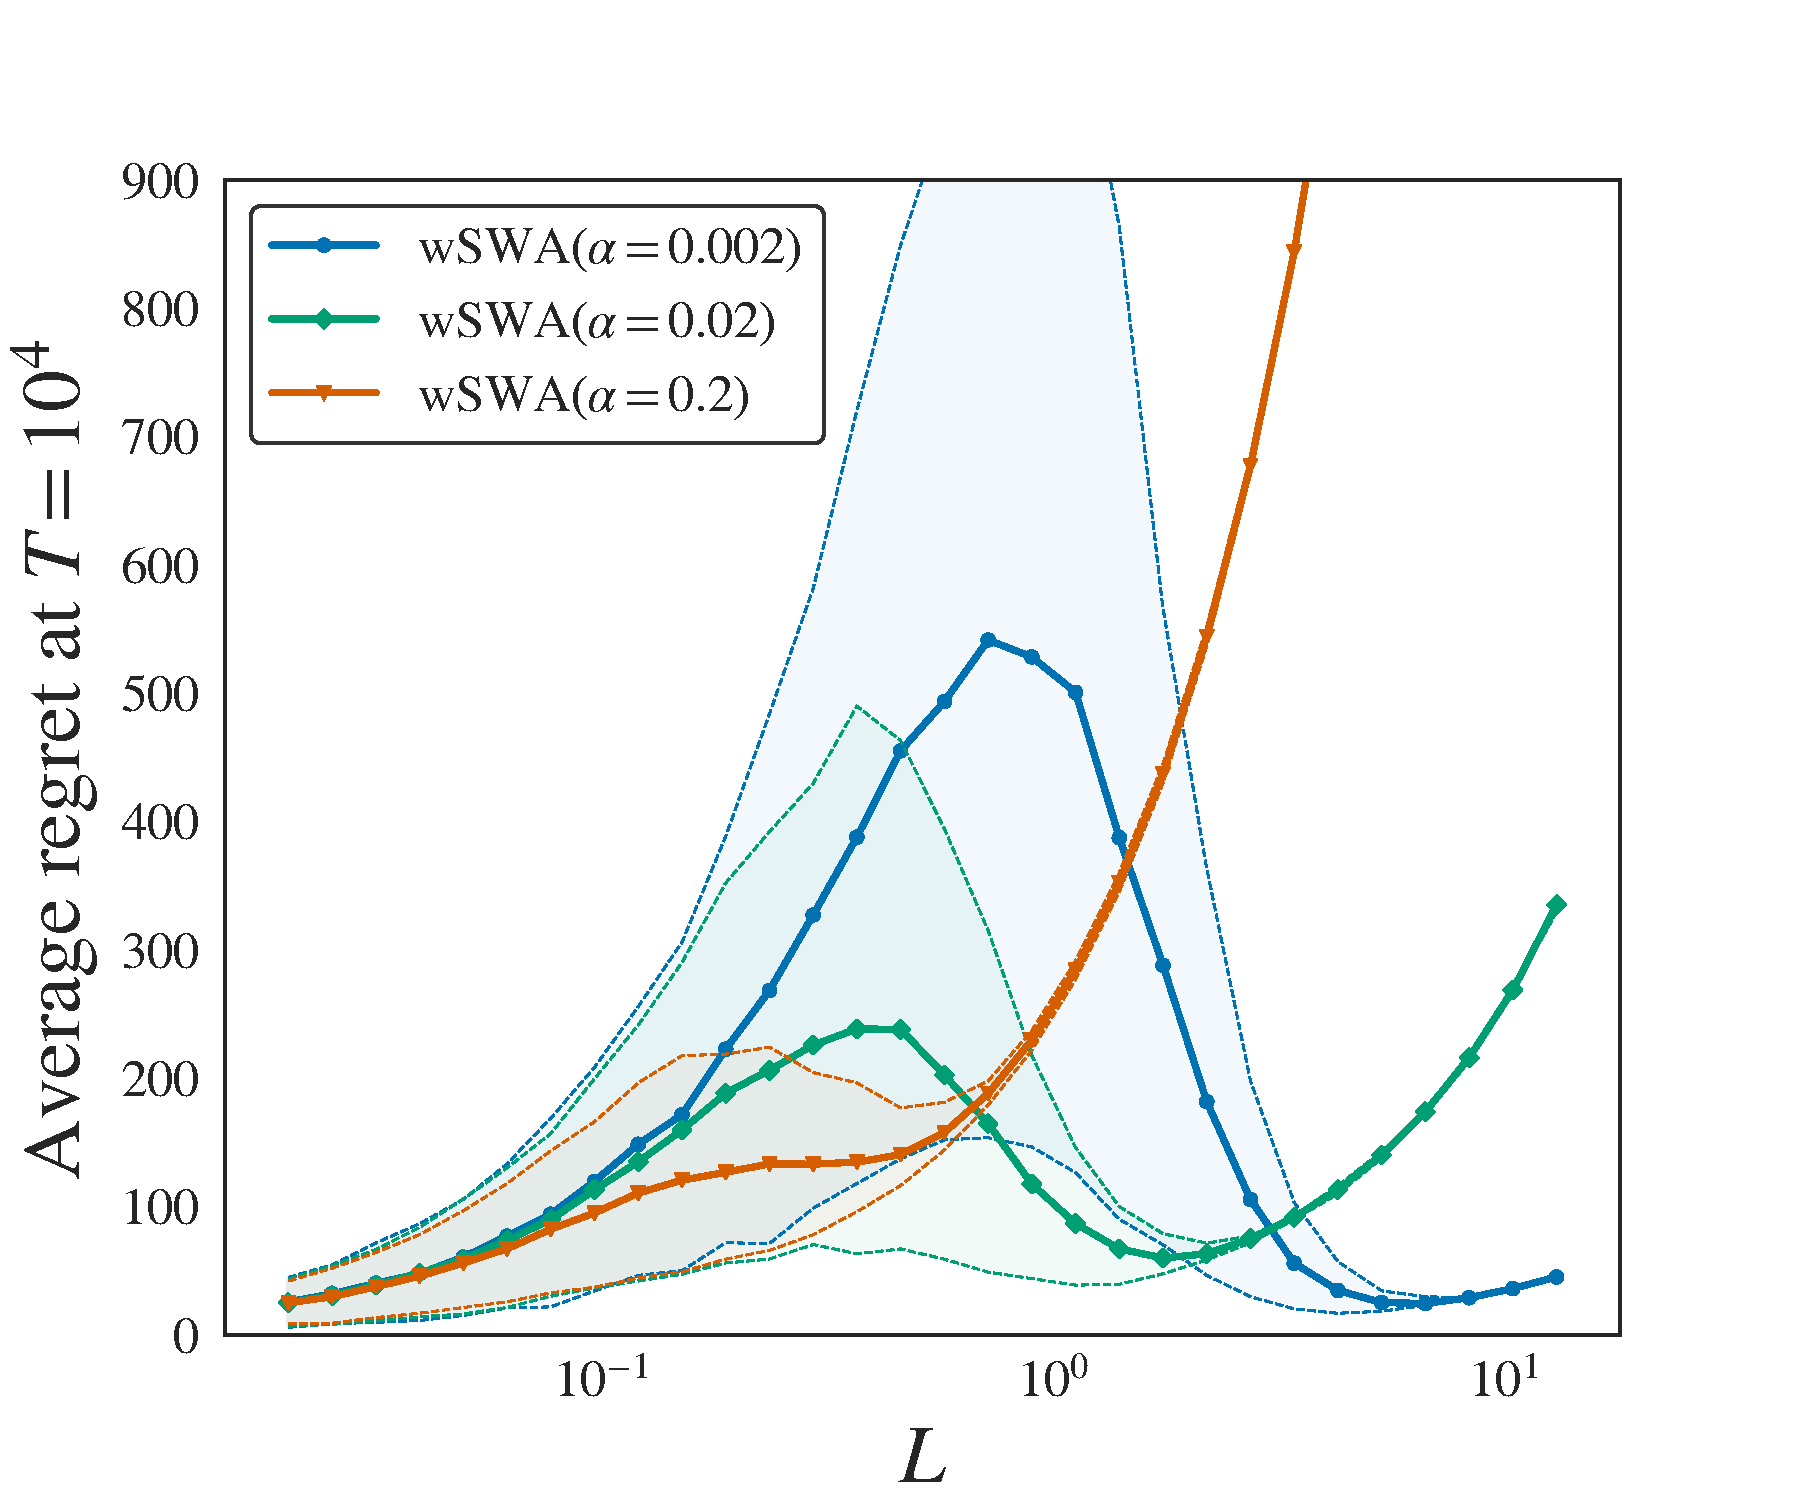
\includegraphics[clip, width= 0.51\textwidth]{2.1Rested/fig/fig1A_SWA.pdf}
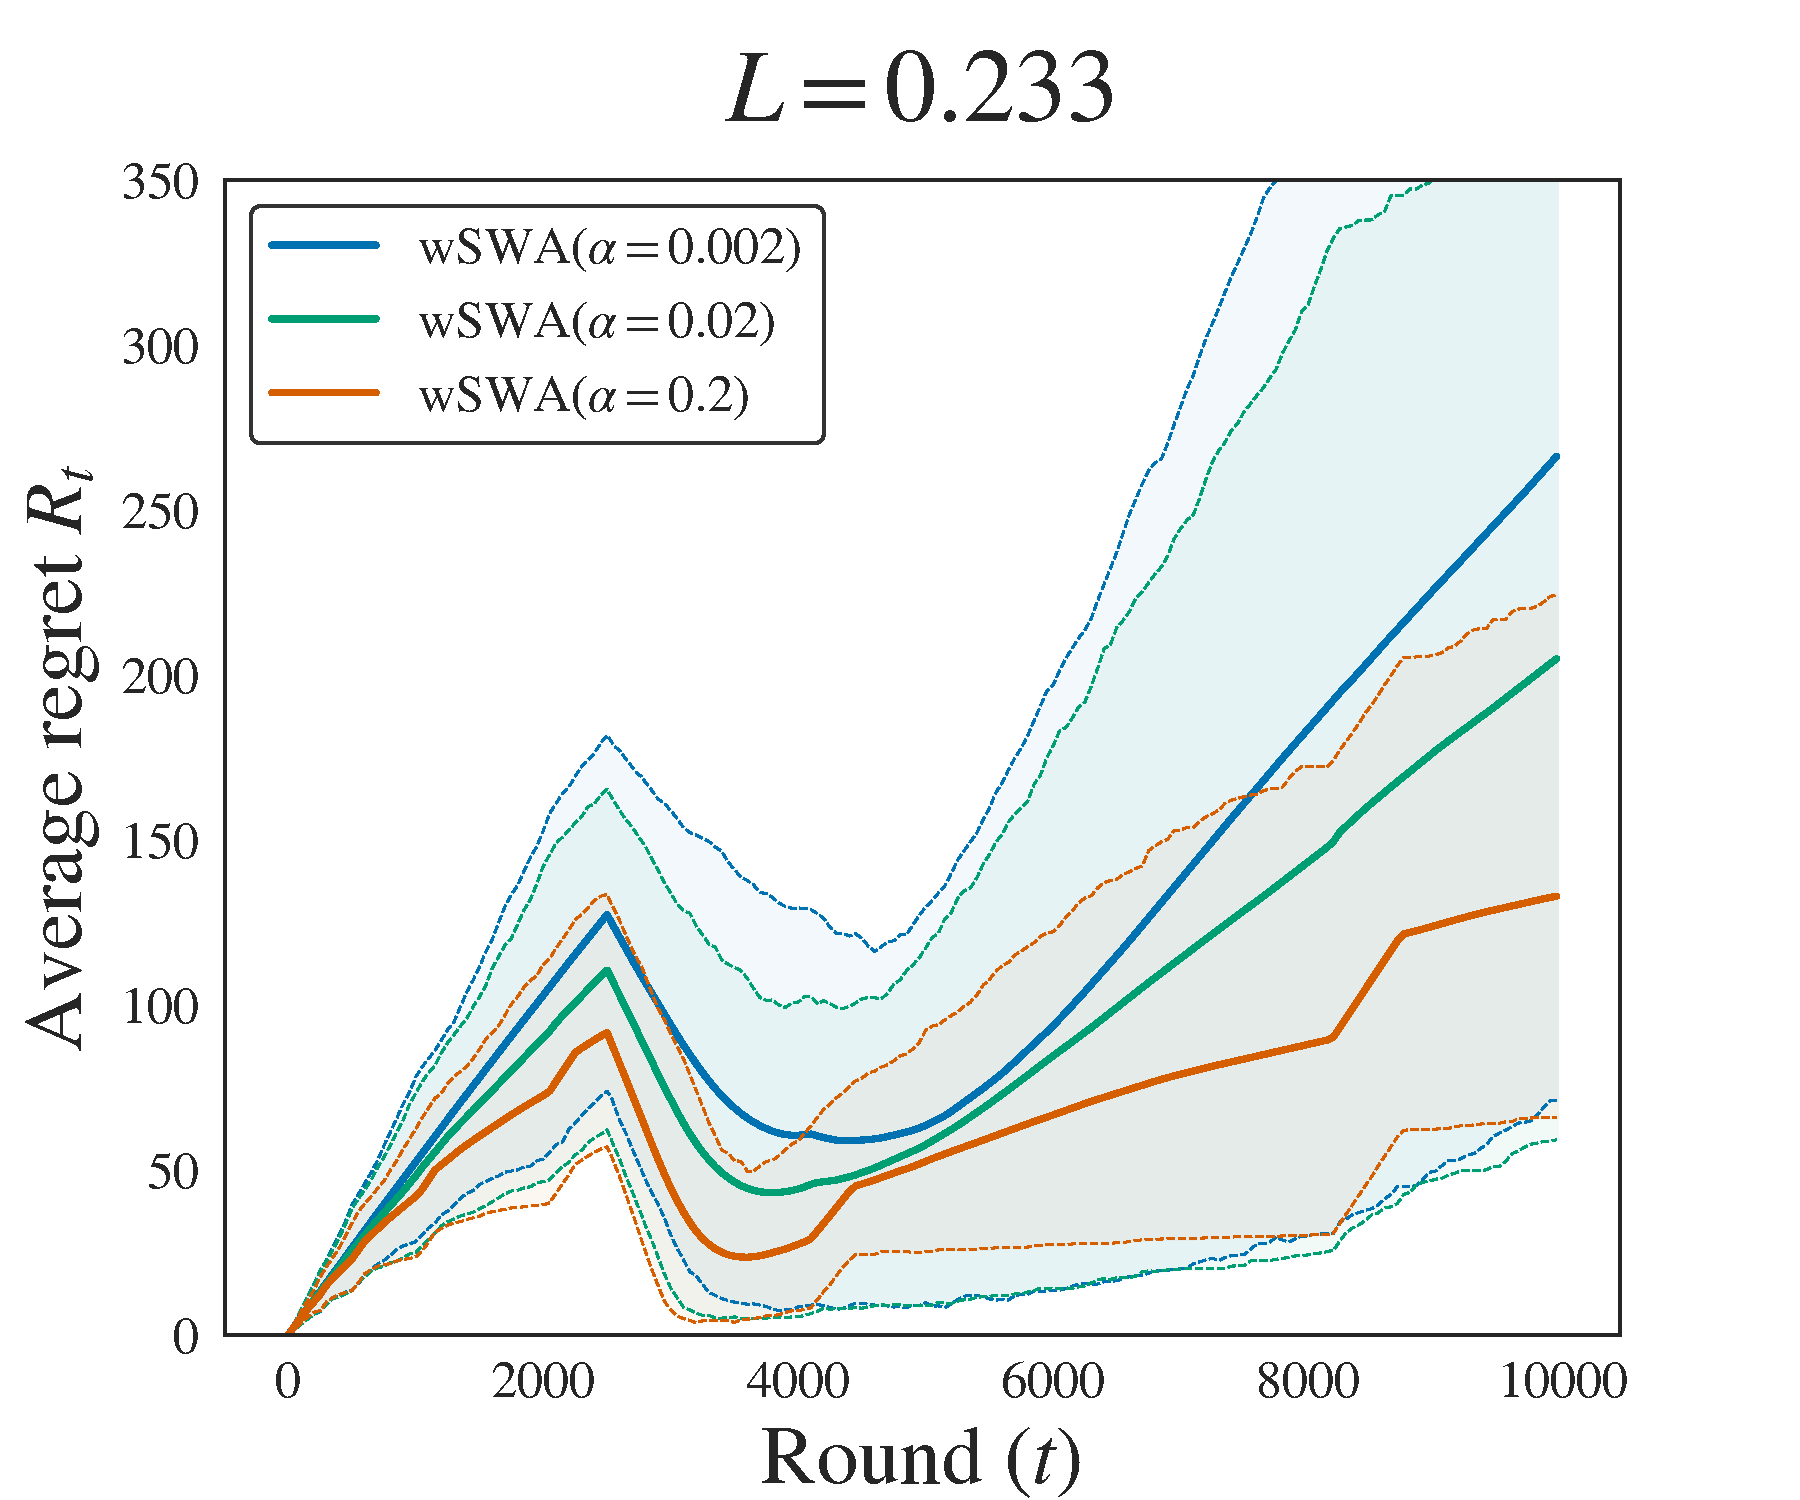
\includegraphics[clip, width= 0.49\textwidth]{2.1Rested/fig/fig1B_SWA.pdf}
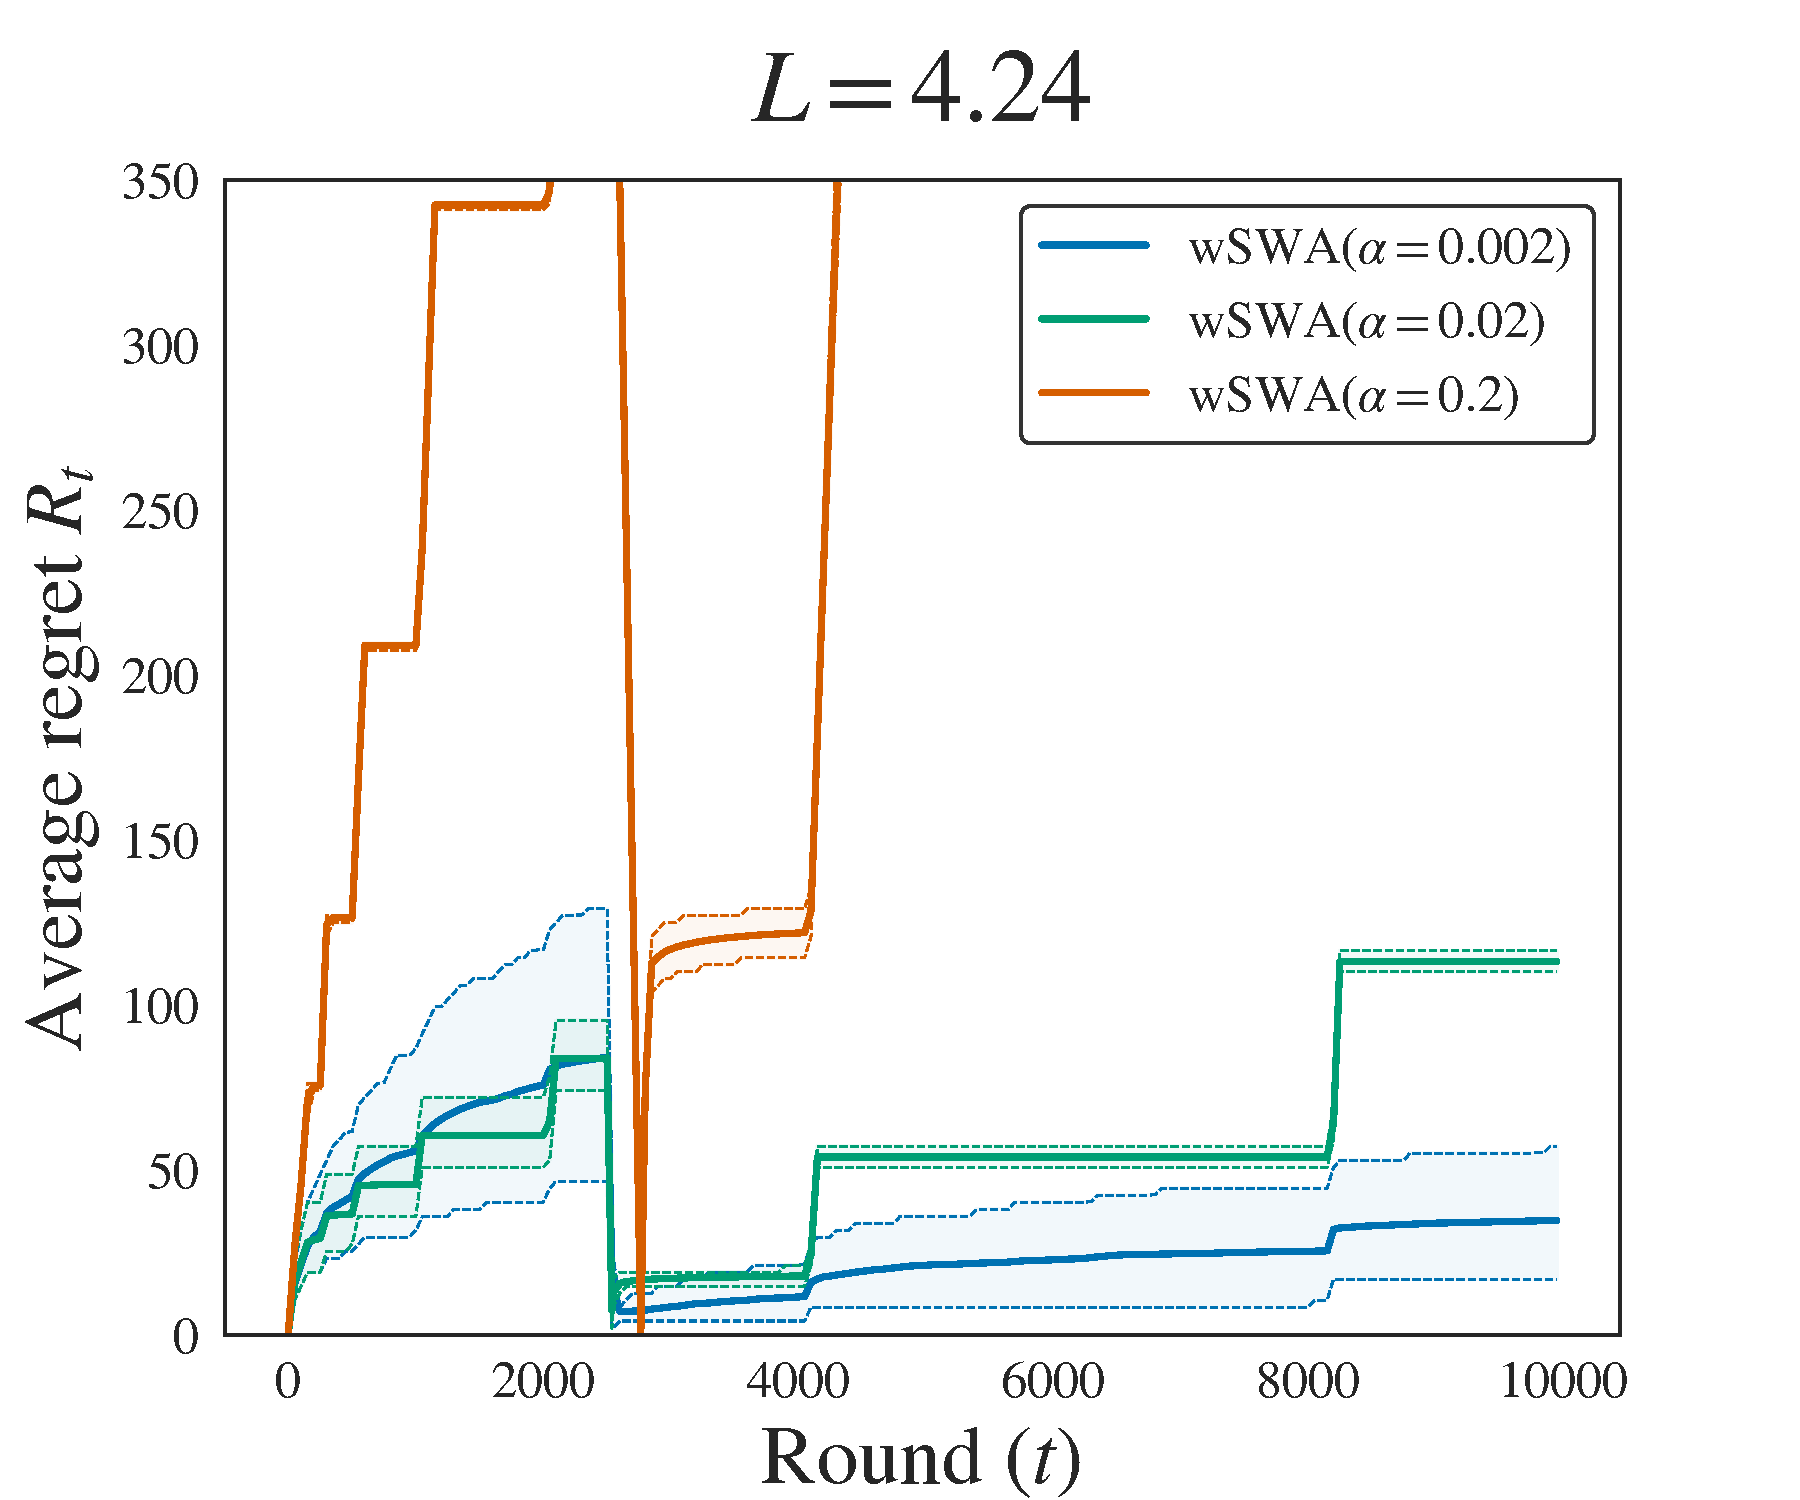
\includegraphics[clip, width= 0.49\textwidth]{2.1Rested/fig/fig1C_SWA.pdf}
\caption{\textbf{Top:} Regret at the end of the game for different values of $L$. \textbf{Bottom:} Regret across time for two values of $L$. Average over 1000 runs. We highlight the $\left[10\%, 90\%\right]$ confidence region.}
\label{fig:SWA1}
\end{figure*}


\paragraph{Results} 
%All experiments are averaged over $1000$ runs.
In Fig.\,\ref{fig:SWA1}, we compare the performance of the three versions of \wSWA. The top plot shows the regret at the last round $T = 10 000$ for 30 different values of~$L$. The bottom plots show the regret as a function of time for $L = 0.233$ and $L=4.24$.  

Each curve of the top plot has three different parts. First, we observe a linear increase for small values of $L$ (exponential shape on the semi-log plot). Indeed, when $\Delta = \nicefrac{L}{2} \lesssim \nicefrac{\sigma}{\sqrt{h}}$, the variance of the indexes are greater than the gap between arms. Therefore, the algorithms are unable to consistently choose the good arm and they do $\cO\pa{T}$ mistakes of size $\Delta$. Hence, the regret grows linearly with $\cO\pa{T\Delta}$ and ultimately with $L$. 

Then, the regret stagnates (red curve) or sharply decreases (green and blue curve). When $\Delta \gtrsim \nicefrac{\sigma}{\sqrt{h}}$, the variance of the indexes is smaller than the gap between arms. Hence, the number of mistakes decrease at an exponential rate with $L^2$ (according to Hoeffding inequality) from $\cO\pa{T}$ to $\tcO\pa{h}$. Notice that there is indeed a factor $\sqrt{\nicefrac{\alpha_{blue}}{ \alpha_{green}}} \sim 3$ between the x-coordinate of the green and blue peaks: it matches the order of magnitude of $L_{peak} \sim  \nicefrac{\sigma}{\sqrt{h}}$.

Yet, in this setup, the concentration of the index can only reduce the number of overpulls of arm $2$ up to $\sim \nicefrac{h}{2}$. Indeed, the expected value of the index of arm $2$ is larger than the expected value of the index of arm $1$ until we do $\nicefrac{h}{2}$ overpulls of arm $2$ because of the bias caused by the pulls before the breakpoint. Moreover, at each restart of the algorithm, both arms are pulled $h$ times. Thus, the regret is lower-bounded by $\tcO\pa{Lh}$ for any $L$ due to the doubling trick restart and the bias of the index. That is why we observe a linear increase (exponential shape on the semi-log plot) of the regret at the end of the green and red curves. Notice that there is a factor 10 between the red and green curves for large values of $L$, which confirms the $\cO\pa{Lh}$ regret rate. We highlight that the red curve does not decrease because this exponential increase takes over the decrease due to the concentration of the index.

The bottom plots show the evolution of the regret for two different values of $L$. We notice that the regret first increases, then decreases at $t = \ceil{\nicefrac{T}{4}}$  and increase again. The regret decreases because at $t = \ceil{\nicefrac{T}{4}}$ the arms' value for the optimal policy are $0$ and $-\nicefrac{L}{2}$  while any sub-optimal policy can obtain either $0$ or $+\nicefrac{L}{2}$. Therefore, the regret cannot increase until \wSWA has pulled arm $2$ for $\floor{\nicefrac{T}{4}}$ times. At this round, the regret is $0$ because we are at the optimal pulling allocation. Notice that we display the expected regret, which might not be equal to $0$ because the different runs do not reach $0$ at the same round.  After that, the regret increases again as \wSWA may select arm $2$ with sub-optimal value $-\nicefrac{L}{2}$.

For $L=0.233$, $\alpha= 0.2$ is the best tuning. Indeed, the difference between arms is only of $\Delta = 0.1$ which is small compared to $\sigma =1$. Therefore, we need a reasonably large averaging window to decrease the variance of the indexes below the gaps between arms, \ie $h \sim \nicefrac{\sigma^2}{\Delta^2} \sim 100$ which is the order of magnitude when $\alpha = 0.2$ ($h=272$ at the end of the game). For $L = 4.24$, $\alpha=0.002$ is the best tuning. Indeed, following the same reasoning, we need $h \sim 1$ which is coherent with $h=3$ at the end of the game when $\alpha = 0.002$.

At each full restart due to the doubling trick wrapper, the two arms are pulled $h$ times which generates $\nicefrac{hL}{2}$ extra regret. The cost of this operation is particularly prohibitive when either $h$ or $L$ is large. For instance, when $L=4.24$, we see periodic sharp increments in the regret when $t=2^i$, especially for the larger values of $\alpha$.


\subsubsection{Simulated benchmark $\#$2: Learning against several drops (10 arms)}
\paragraph{Experiments.} We also tested a rotting setting with 10 arms. The mean of 1 arm is constant with value 0 while the means of 9 arms abruptly decrease after 1000 pulls from $+\Delta_i$ to $-\Delta_i$. We use nine different values of $\Delta_i$ which are ranging from 0.001 to 10 in a geometric sequence. In this setting, the regret can be written as $R_T(\pi) = \sum_{i=1}^9 h_{i,T}\Delta_i$, with $h_{i,T}$ the number of overpulls of arm $i$ at round $T$. We define the regret per arm, $R_T^i(\pi) \triangleq \Delta_i h_{i,T}$.

\paragraph{Algorithms.} We keep the three versions of \wSWA with $\alpha \in \left\{ 0.002, 0.02, 0,2\right\}$. We add to our benchmark famous stationary, adversarial and non-stationary algorithms: \UCB \citep{lai1985asymptotically}, \EXP, \EXPS \citep{auer2002nonstochastic}, \DUCB, \SWUCB \citep{garivier2011upper-confidence-bound} and \GLRUCB \citep{besson2019generalized}. 

For $\UCB$ we use the asymptotic optimal tuning of the confidence bounds for stationary gaussian bandits. For $\EXP$ and $\EXPS$, we use theoretical tuning using the number of breakpoints and the horizon. For \SWUCB and \DUCB, we select the forgetting parameters $\tau=200$ and $\gamma = 0.997$ with grid-search for best performance on this problem. For \GLRUCB, we use the theoretical value $\delta = \sqrt{T}^{-1}$ for the change-point sensitivity and we set the probability of random exploration to $0$. Indeed, the random exploration is used to detect (restless) increment in the sub-optimal arms value which is irrelevant for our rested rotting setup.


\begin{figure*}[t]
\centering
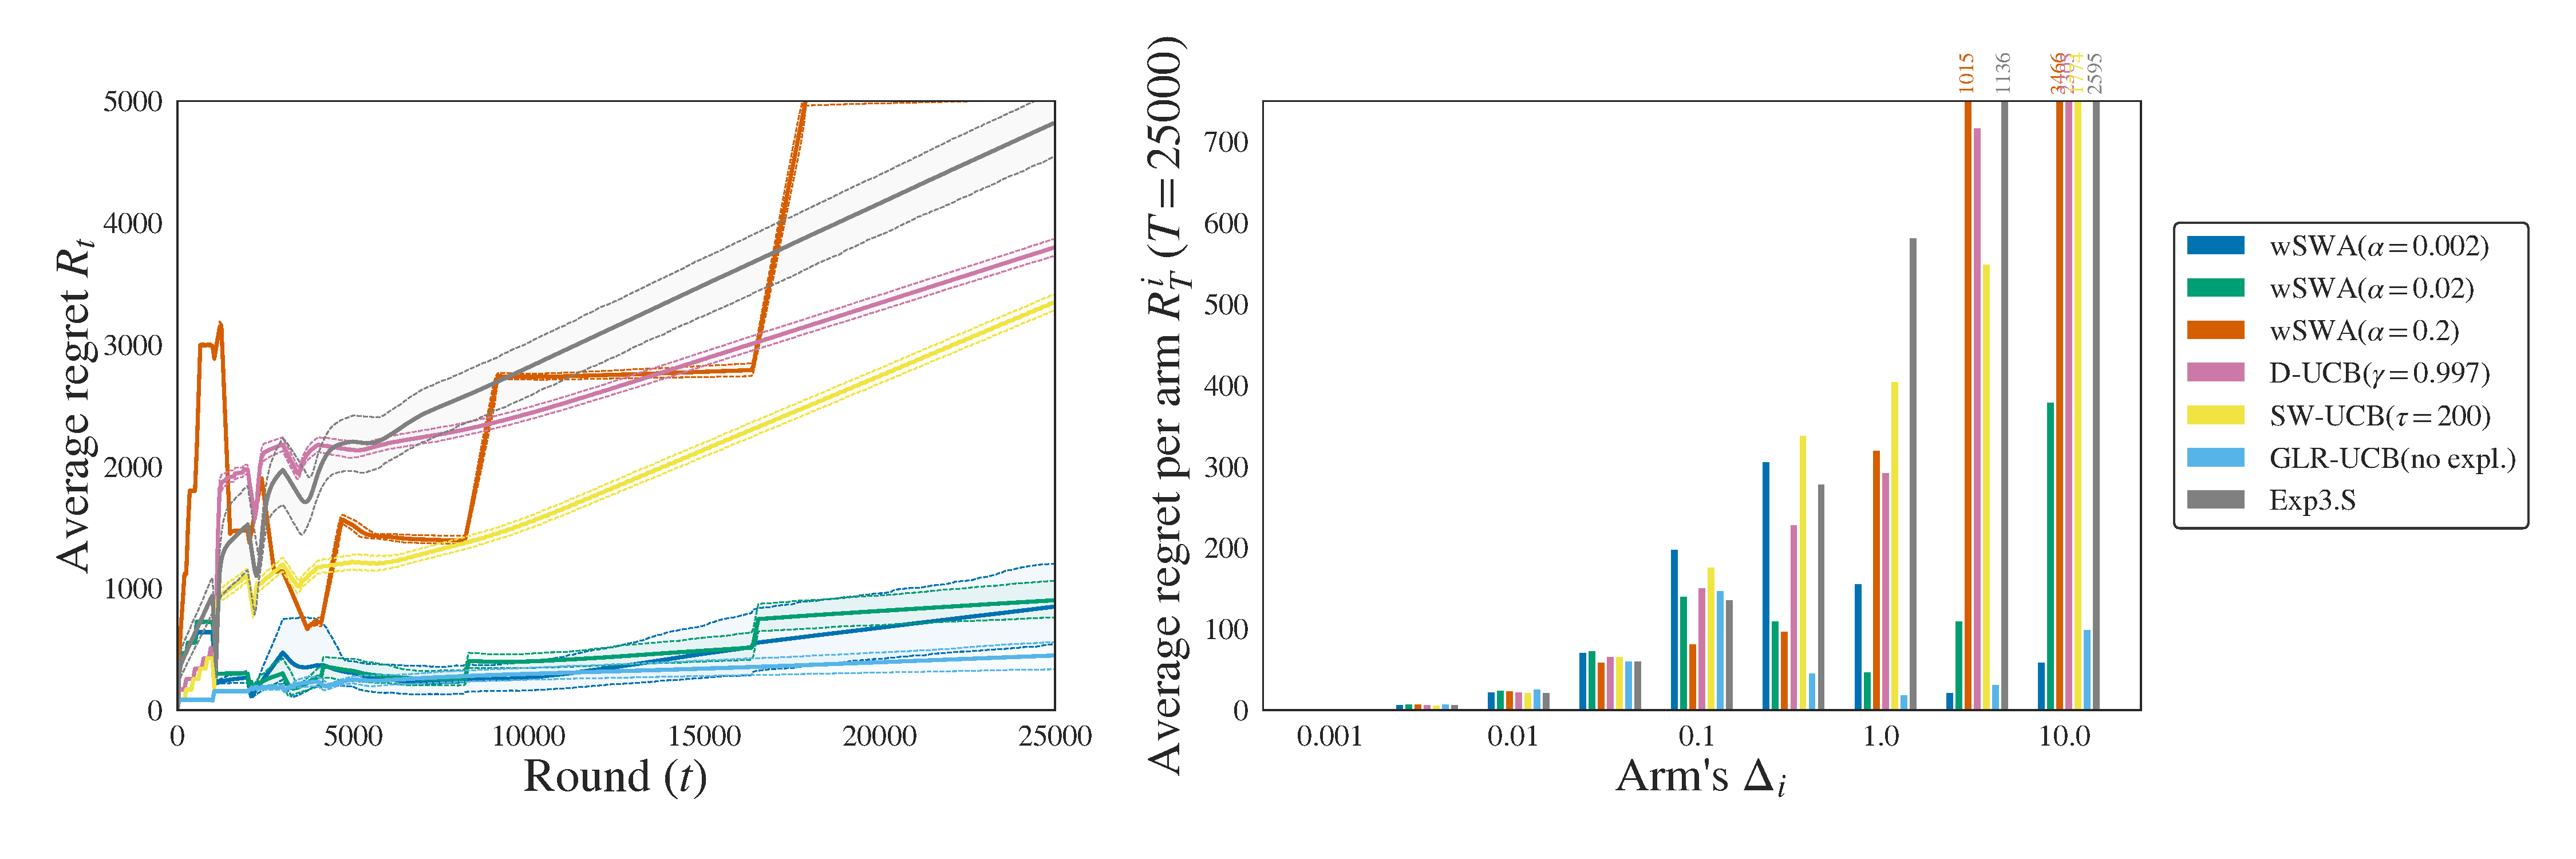
\includegraphics[width = 0.99 \textwidth]{2.1Rested/fig/fig2_SWA.pdf}
\caption{\textbf{Left:} Regret at the end of the game for different values of $L$. \textbf{Middle, Right:} Regret across time for two values of $L$. Average over 1000 runs. We highlight the $\left[10\%, 90\%\right]$ confidence region.}
\label{fig:SWA2}
\end{figure*}

\paragraph{Results.} We display the average regret through the rounds and the regret per arm at the end of the horizon in Figure~\ref{fig:SWA2}.

We do not display the results for \UCB and \EXP because they obtain very large regret after the first drop in the reward (~20 000 at the end of the game). Indeed, these two algorithms are designed for the fixed-arm regret and are unable to adapt to change of the best arm identity. 
 
\SWUCB, \DUCB, and \EXPS show large regret even though \SWUCB and \DUCB were optimally tuned for this problem. These algorithms use random exploration and/or restless forgetting of the data associated with each arm. This is harmful because it leads to multiple pulls of a very suboptimal arm. Yet, with the rested rotting non-stationarity, an identified bad arm has no reason to improve.
 
\SWA shows better performance when it is rightly tuned. In this problem, we have multiple sizes of drops and one should choose a value $\alpha$ which trades-off between these different sizes.  $\alpha=0.2$, which obtains the best value in \citet{levine2017rotting}'s experiment, has a very large regret in our benchmark. Indeed, the best tuning depends on the maximal size of the drops, which is quite large in our setting. We also notice the cost of the doubling trick.

Last, \GLRUCB shows good performance when random exploration is turned off. Indeed, the change detection mechanism reset the history of the arm when there is significant evidence of a change. Hence, the number of mistakes after a drop is adaptive to the difficulty to detect the change. 

\subsection{Open problems}
\label{subsec:rested-open}
\subsubsection{Minimax rate}
We report existing regret bounds for two special cases. First, in Proposition~\ref{prop:lb-noisefree}, \citet{heidari2016tight} show that in the absence of noise, the regret is lower bounded by $\cO\pa{KL}$. Second, we recall the minimax regret lower bound for stochastic stationary bandits.

\begin{proposition}[\cite{auer2002nonstochastic}][Thm.\,5.1]
\label{stochastic-LB}
For any learning policy $\policy$ and any horizon $T$, there exists a stochastic stationary problem $\left\{ \mu_i (n) \triangleq \mu_i\right\}_i$ with $K$ $\sigma$-sub-gaussian arms such that $\pi$ suffers a regret
\begin{equation*}
%\max_{\left\{ \mu_i \in [0,L] \right\}_i}
 \mathbb{E}[\regret(\policy)] \geq \frac{\sigma}{10}\min\pa{\sqrt{\narms\timeEnd},\timeEnd}.
\end{equation*}
where the expectation is w.r.t.\ both the randomization
over rewards and algorithm's internal randomization.
\end{proposition}

Any problem in the two settings above is a rotting problem with parameters ($\sigma$, $L$). Therefore, the performance of any algorithm on the noisy rotting problem is also bounded by these two lower bounds. For reward functions in $\BBSet$, \SWA is guaranteed to achieve $\cO\pa{T^{\nicefrac{2}{3}}}$ regret rate. Yet, \citet{levine2017rotting} do not provide a lower bound while they suggest it could be an interesting future work direction.

\subsubsection{Problem-dependent rate}
\SWA starts by pulling every arm $h$ times. It means that even for simple stationary problem with large difference $\Delta_i > \sigma$ between suboptimal and optimal arms, \SWA makes at least $h = \cO\pa{T^{\nicefrac{2}{3}}}$ mistakes per suboptimal arms which is much more than the stationary asymptotic optimal pulling rate $\cO\pa{\nicefrac{\sigma\log\pa{T}}{\Delta_i^2}}$.


\subsubsection{Agnostic algorithm}
\SWA requires the knowledge of the horizon $T$, the subgaussian parameter $\sigma$, and the reward range $B$  to tune the window $h$. We showed empirically that the doubling trick leads to large regret increases at each restart. We also show that not knowing the amplitude of the drops $B$ could lead to very suboptimal tuning.

\begin{remark}
\citet{levine2017rotting} suggest in \wSWA to use the classical doubling trick, with a full restart of the memory of the algorithm. It is an easy way to generalize the $\tcO\pa{T^{\nicefrac{2}{3}}}$ bound when we do not know $T$. However, in practice, in this rested setup, there is no good reason to clean the memory of \wSWA (see Line~\ref{algline:wSWA-clean}). We could simply increase the window $h$ and keep the current history of the arms in order to diminish the cost of the restart. The empirical investigation of this algorithm showed improved results compared to \wSWA without completely removing the extra cost of the doubling trick.
\end{remark}


\subsubsection{Global budget or Budget per round}

The analysis of \SWA was carried in the global rotting budget setting while the analysis of the noiseless case was carried in the per round budget setting. We can translate the $\tcO\pa{B^{\nicefrac{1}{3}}T^{\nicefrac{2}{3}}}$ bound by setting $B= LT$ which leads to linear regret (see the remark following Definition~\ref{def:rew-bounded}). Hence, no algorithm is proved to achieve a $o(T)$ regret bound in the rotting budget per round setting with noise.
